\begin{frame}
  \titlepage

  \vskip-0.5cm

  \centering
  \small{
    Conferința Anuală de Comunicare a Rezultatelor Cercetării la UB
  }

  \vskip0.1cm
\end{frame}

\section{Introducere}

\begin{frame}
  \frametitle{Motivație}

  \begin{itemize}
    \item Lumina este o \textbf{oscilație transversă} a câmpului electromagnetic.
    \item La fel ca orice undă transversă, poate avea \textbf{moment cinetic} (\textit{angular momentum}), pe care îl descompunem într-o componentă datorată polarizării (\textbf{moment cinetic de spin}) și una datorată formei frontului de undă (\textbf{moment cinetic orbital}).
  \end{itemize}
\end{frame}

\begin{frame}
  \frametitle{Momentul cinetic al luminii}

  \begin{figure}
    \centering
    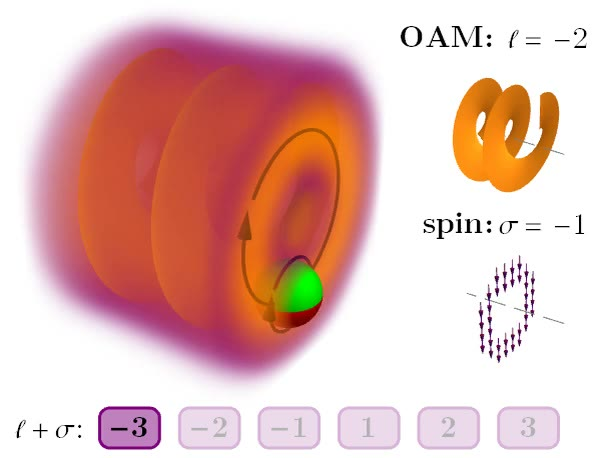
\includegraphics[width=0.75\textwidth]{figures/oam_vs_spin.jpg}
    \caption{Cadru dintr-un video de pe \href{https://en.wikipedia.org/wiki/File:OAM_vs_spin_video.ogg}{Wikipedia}, creat de Jozum Bjada}
  \end{figure}
\end{frame}

\begin{frame}
  \frametitle{Schema experimentală}

  \begin{figure}
    \centering
    \resizebox{\columnwidth}{!}{\inputtikz{figures/experiment_geometry.tex}}
    \caption{Reprezentare vizuală a metodei propuse. Un fascicul laser LG care se propagă în direcția \(-z\) lovește un mănunchi de electroni relativiști care se mișcă în direcția \(+z\). Radiația emisă este măsurată pe un detector aflat la o distanță \(Z\).}
  \end{figure}
\end{frame}

\begin{frame}
  \centering{
    \huge{Mulțumesc pentru atenție!}
  }
\end{frame}

\begin{frame}[allowframebreaks]
  \frametitle{Referințe}

  \printbibliography
\end{frame}

\section{Backup slides}

\begin{frame}
  \frametitle{Ecuațiile lui Maxwell}

  Undele pe care le studiem sunt soluții ale \textbf{ecuațiilor lui Maxwell} \cite{Maxwell1865,Jackson1999,Griffiths2023}:

  \begin{align*}
    &\symbf{\nabla} \cdot \symbf{E} = \frac{\rho}{\epsilon_0} \tag{Legea lui Gauss} \\[0.2em]
    &\symbf{\nabla} \times \symbf{E} = - \frac{\partial \symbf{B}}{\partial t} \tag{Legea lui Faraday} \\[0.2em]
    &\symbf{\nabla} \cdot \symbf{B} = 0 \\[0.2em]
    &\symbf{\nabla} \times \symbf{B} = \mu_0 \symbf{J} + \mu_0 \epsilon_0 \frac{\partial \symbf{E}}{\partial t} \tag{Ampère-Maxwell} \\[0.2em]
    &\symbf{F} = q \left(\symbf{E} + \symbf{v} \times \symbf{B}\right) \tag{Forța Lorentz}
  \end{align*}
\end{frame}
